This section visualize the result from the linear regressions, and the performance of the deep learning models using multiple pain maps representation, and different outputs. 

\begin{figure*} [b!]
\begin{tcolorbox}[colframe=black!30!black, colback=white]
\hfill
\begin{subfigure}[r]{0.5\textwidth}
    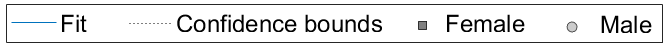
\includegraphics[width=\textwidth]{Figures/legend}
  \end{subfigure}
  \vskip\baselineskip
  \hspace{-5mm}
  \begin{subfigure}[b]{0.51\textwidth}
    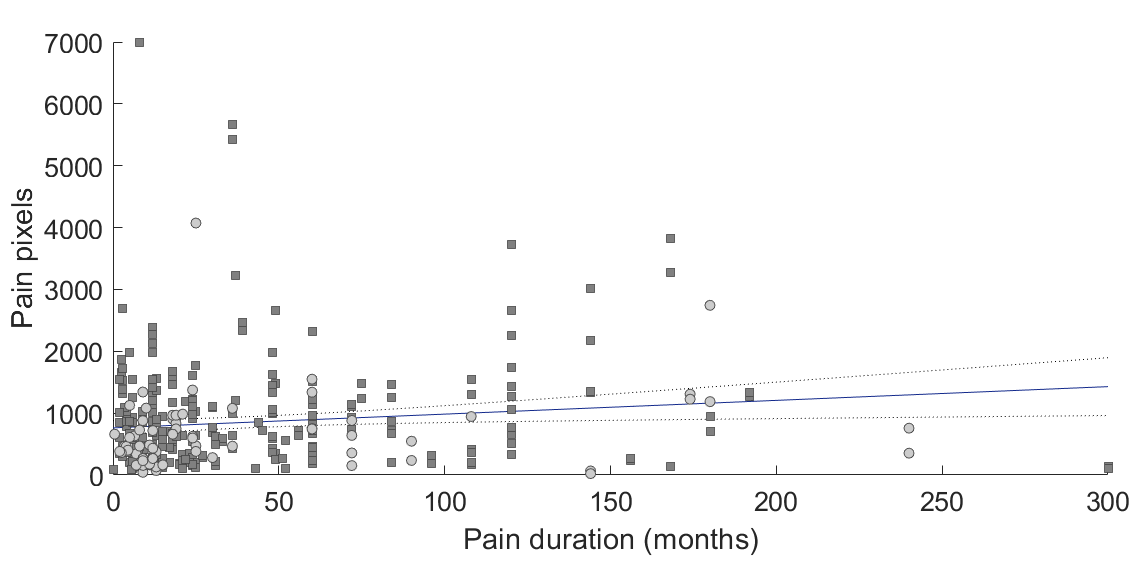
\includegraphics[width=\textwidth]{Figures/durapixel}
    \caption{ }
    \label{fig:1}
  \end{subfigure}
  \hfill
    \hspace{2mm}
  \begin{subfigure}[b]{0.51\textwidth}
    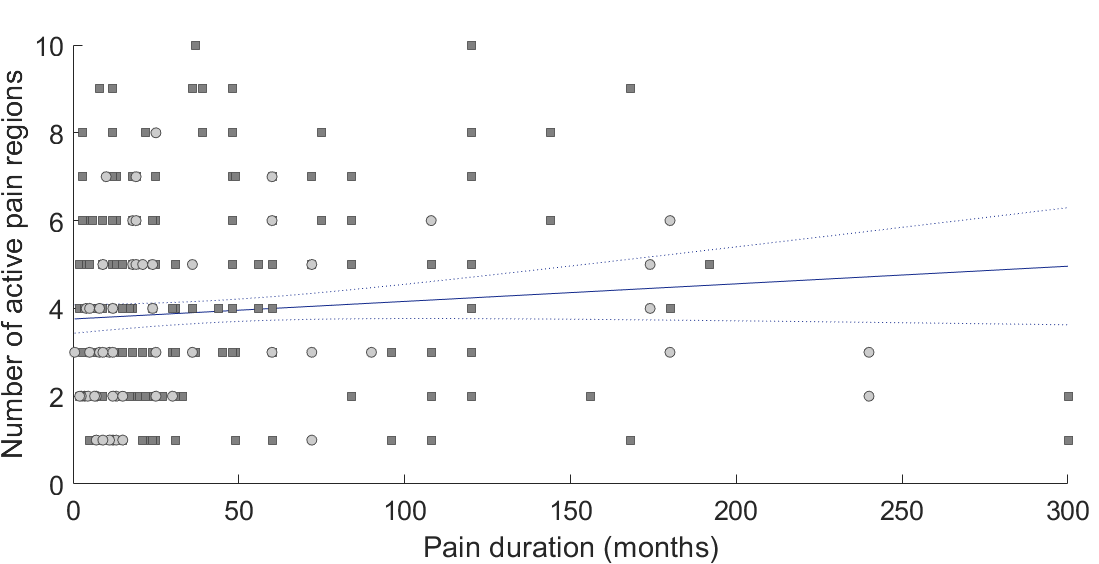
\includegraphics[width=\textwidth]{Figures/duraregion}
       \caption{ }
    \label{fig:2}
  \end{subfigure}
    \vskip\baselineskip
    \hspace{-5mm}
  \begin{subfigure}[b]{0.51\textwidth}
    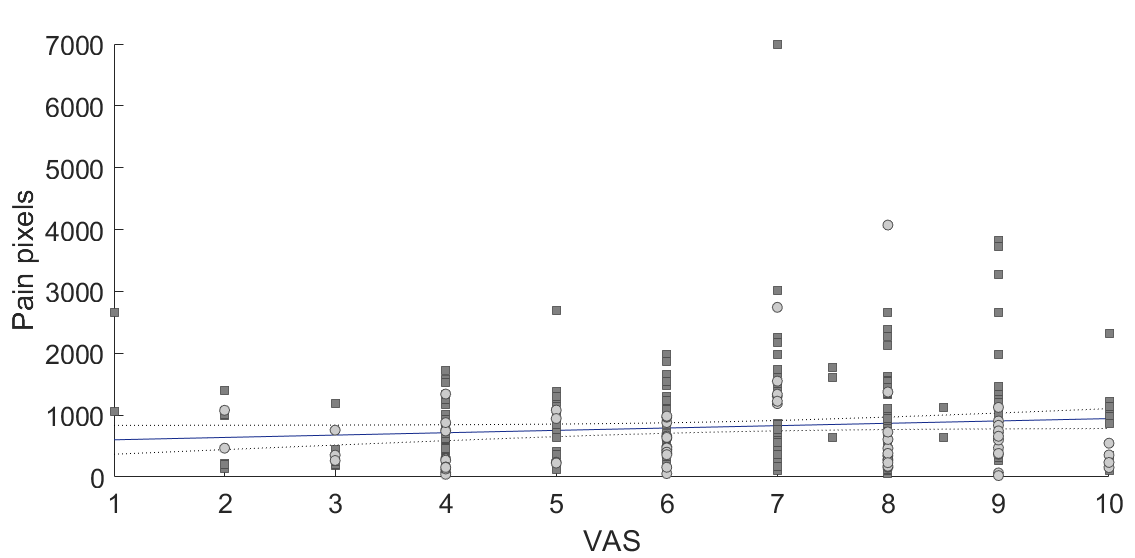
\includegraphics[width=\textwidth]{Figures/vaspixel}
    \caption{}
    \label{fig:3}
  \end{subfigure}
  \hfill
  \hspace{2mm}
  \begin{subfigure}[b]{0.51\textwidth}
    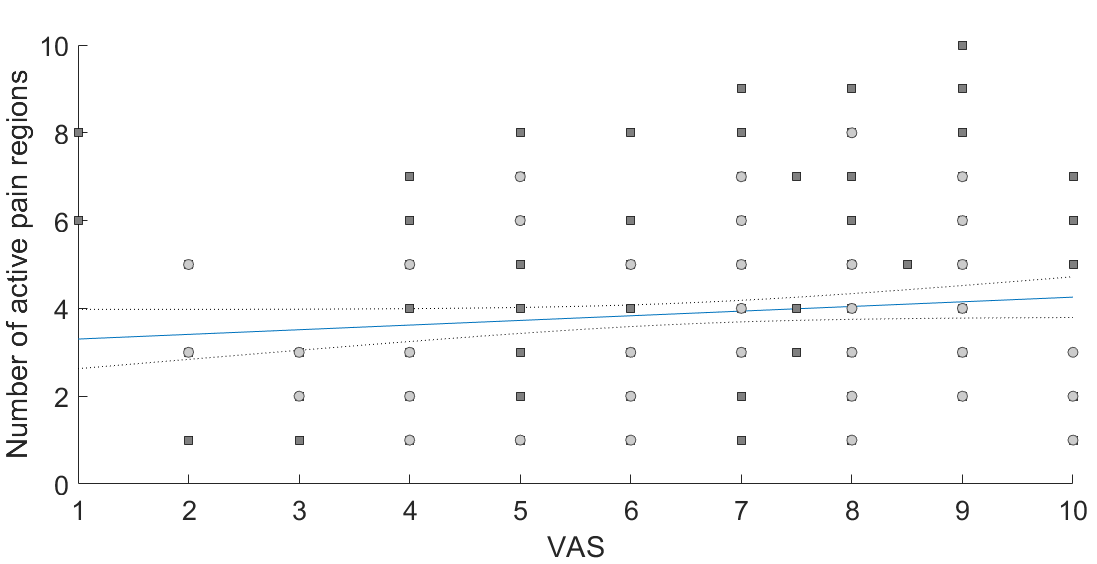
\includegraphics[width=\textwidth]{Figures/vasregion}
       \caption{ }
    \label{fig:4}
  \end{subfigure}  
  \caption{Linear correlations of pain pixels and pain duration (a), active pain regions and pain duration (b), pain pixels and pain intensity indicated in VAS (c), and active pain regions and pain intensity indicated in VAS (d).}
  \label{fig:correlations}
\end{tcolorbox}
\end{figure*}

\subsection*{Linear correlations}
The linear regression between simple features, number of pain pixels or active pain regions, and outputs, pain duration or pain intensity, resulted in the plots shown in fig. \ref{fig:correlations}. The $R^2$-values support the nonlinearity, shown in the plots, where correlation fig. \ref{fig:1} resulted in a $R^2 = 0.018$, fig. \ref{fig:2} resulted in $R^2 = 0.008$, fig. \ref{fig:3} resulted in $R^2 = 0.011$ and fig. \ref{fig:4} resulted in $R^2 =  0.011$. 

\subsection*{Optimization of the models}
During the optimization, a manual 



\subsection*{Performance of the models}
The average performance accuracy, sensitivity, and specificity of the models during test with new pain maps in different representations are shown in tab. \ref{tab:performance}.

\begin{table*}[b]
\centering
\begin{tabular}{@{}llll@{}}
\toprule
\multicolumn{4}{c}{\hspace{2.3cm} Avg. accuracy (\%) \hspace{1cm} Avg. sensitivity (\%) \hspace{1cm} Avg. specificity (\%) \hspace{1cm}                }                                                                                                                                                                         \\ \midrule
\multicolumn{4}{c}{Morphology-representation} \\ \midrule
Pain duration  & \hspace{0.7cm}\begin{tabular}[c]{@{}l@{}}69.44\% \end{tabular} & \hspace{2.6cm} \begin{tabular}[c]{@{}l@{}}69.23\%\end{tabular} & \hspace{2.7cm} \begin{tabular}[c]{@{}l@{}} 69.57\%\end{tabular} \\ %\midrule
Pain intensity & \hspace{0.6cm} \begin{tabular}[c]{@{}l@{}}60.00\% \end{tabular}  & \hspace{2.7cm}\begin{tabular}[c]{@{}l@{}}40.00\% \end{tabular}  & \hspace{2.7cm} \begin{tabular}[c]{@{}l@{}}70.00\%\end{tabular}   \\ \midrule
\multicolumn{4}{c}{Location-representation}                                                                                                                                                                             \\ \midrule
Pain duration  & \hspace{0.6cm} \begin{tabular}[c]{@{}l@{}}35.29\%\end{tabular}  & \hspace{2.6cm} \begin{tabular}[c]{@{}l@{}}0.00\% \end{tabular}  & \hspace{2.7cm} \begin{tabular}[c]{@{}l@{}}35.29\%\end{tabular}  \\ %\midrule 
Pain intensity & \hspace{0.6cm} \begin{tabular}[c]{@{}l@{}}60.71\% \end{tabular}   & \hspace{2.6cm} \begin{tabular}[c]{@{}l@{}}0.00\% \end{tabular}   & \hspace{2.7cm} \begin{tabular}[c]{@{}l@{}}60.71\%\end{tabular}  \\ \midrule
\multicolumn{4}{c}{Combined-representation}                                                                                                                                                              \\ \midrule
Pain duration  & \hspace{0.6cm} \begin{tabular}[c]{@{}l@{}}55.56\% \end{tabular}                                                                   & \hspace{2.6cm} \begin{tabular}[c]{@{}l@{}}61.11\%\end{tabular}                                                                & \hspace{2.7cm} \begin{tabular}[c]{@{}l@{}}50.00\%\end{tabular}                                                                                                                                \\% \midrule
Pain intensity & \hspace{0.6cm} \begin{tabular}[c]{@{}l@{}}73.33\% \end{tabular}
&\hspace{2.6cm} \begin{tabular}[c]{@{}l@{}} 0\%\end{tabular}                                                               
& \hspace{2.7cm} \begin{tabular}[c]{@{}l@{}} 73.33\%\end{tabular}                                                               
 \\ \bottomrule
\end{tabular}
\caption{Generalization performance of the models, which use the morphology-, location- and combined-representation when classifying according to pain duration or pain intensity.}
\label{tab:performance}
\end{table*}